\chapter{\abstractname}

\begin{figure}[h]
    \centering
    \begin{subfigure}[b]{0.3\linewidth}
      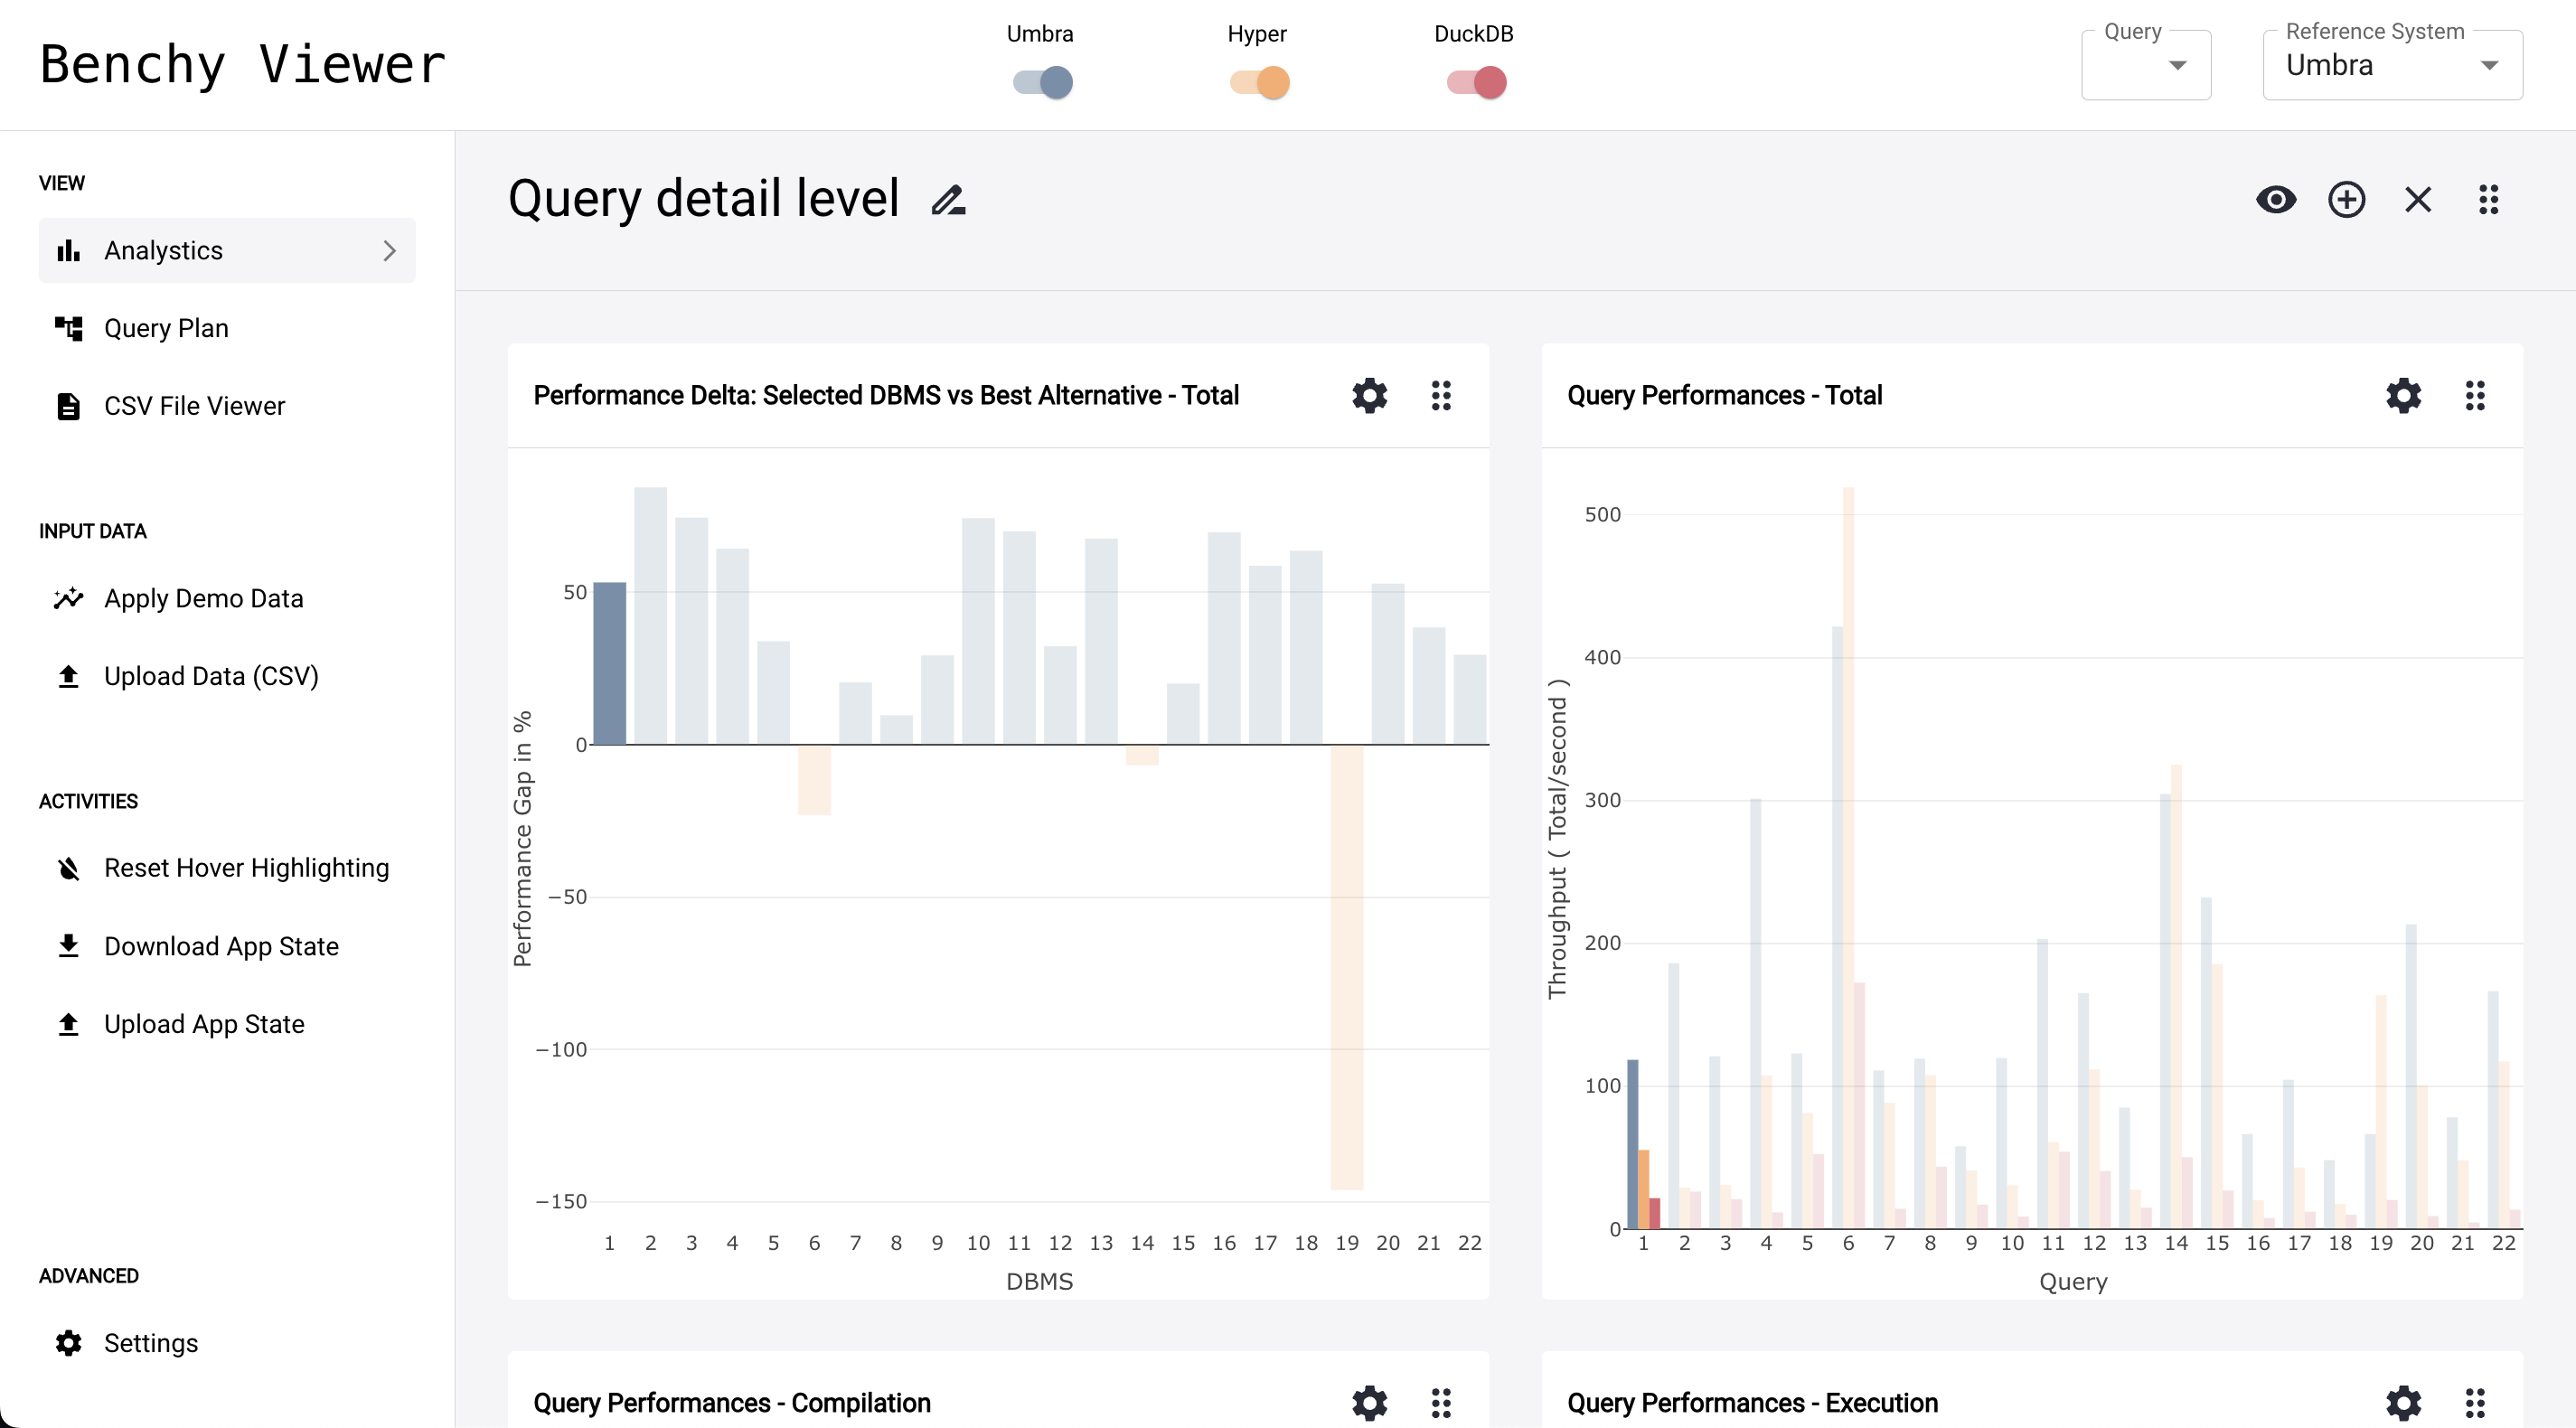
\includegraphics[width=\linewidth]{figures/app.png}
      \caption{Analytics Dashboard.}
        \label{fig:abstract-page}
    \end{subfigure}
    \hspace{0.5cm} % Adjust the horizontal space between the figures
    \begin{subfigure}[b]{0.3\linewidth}
      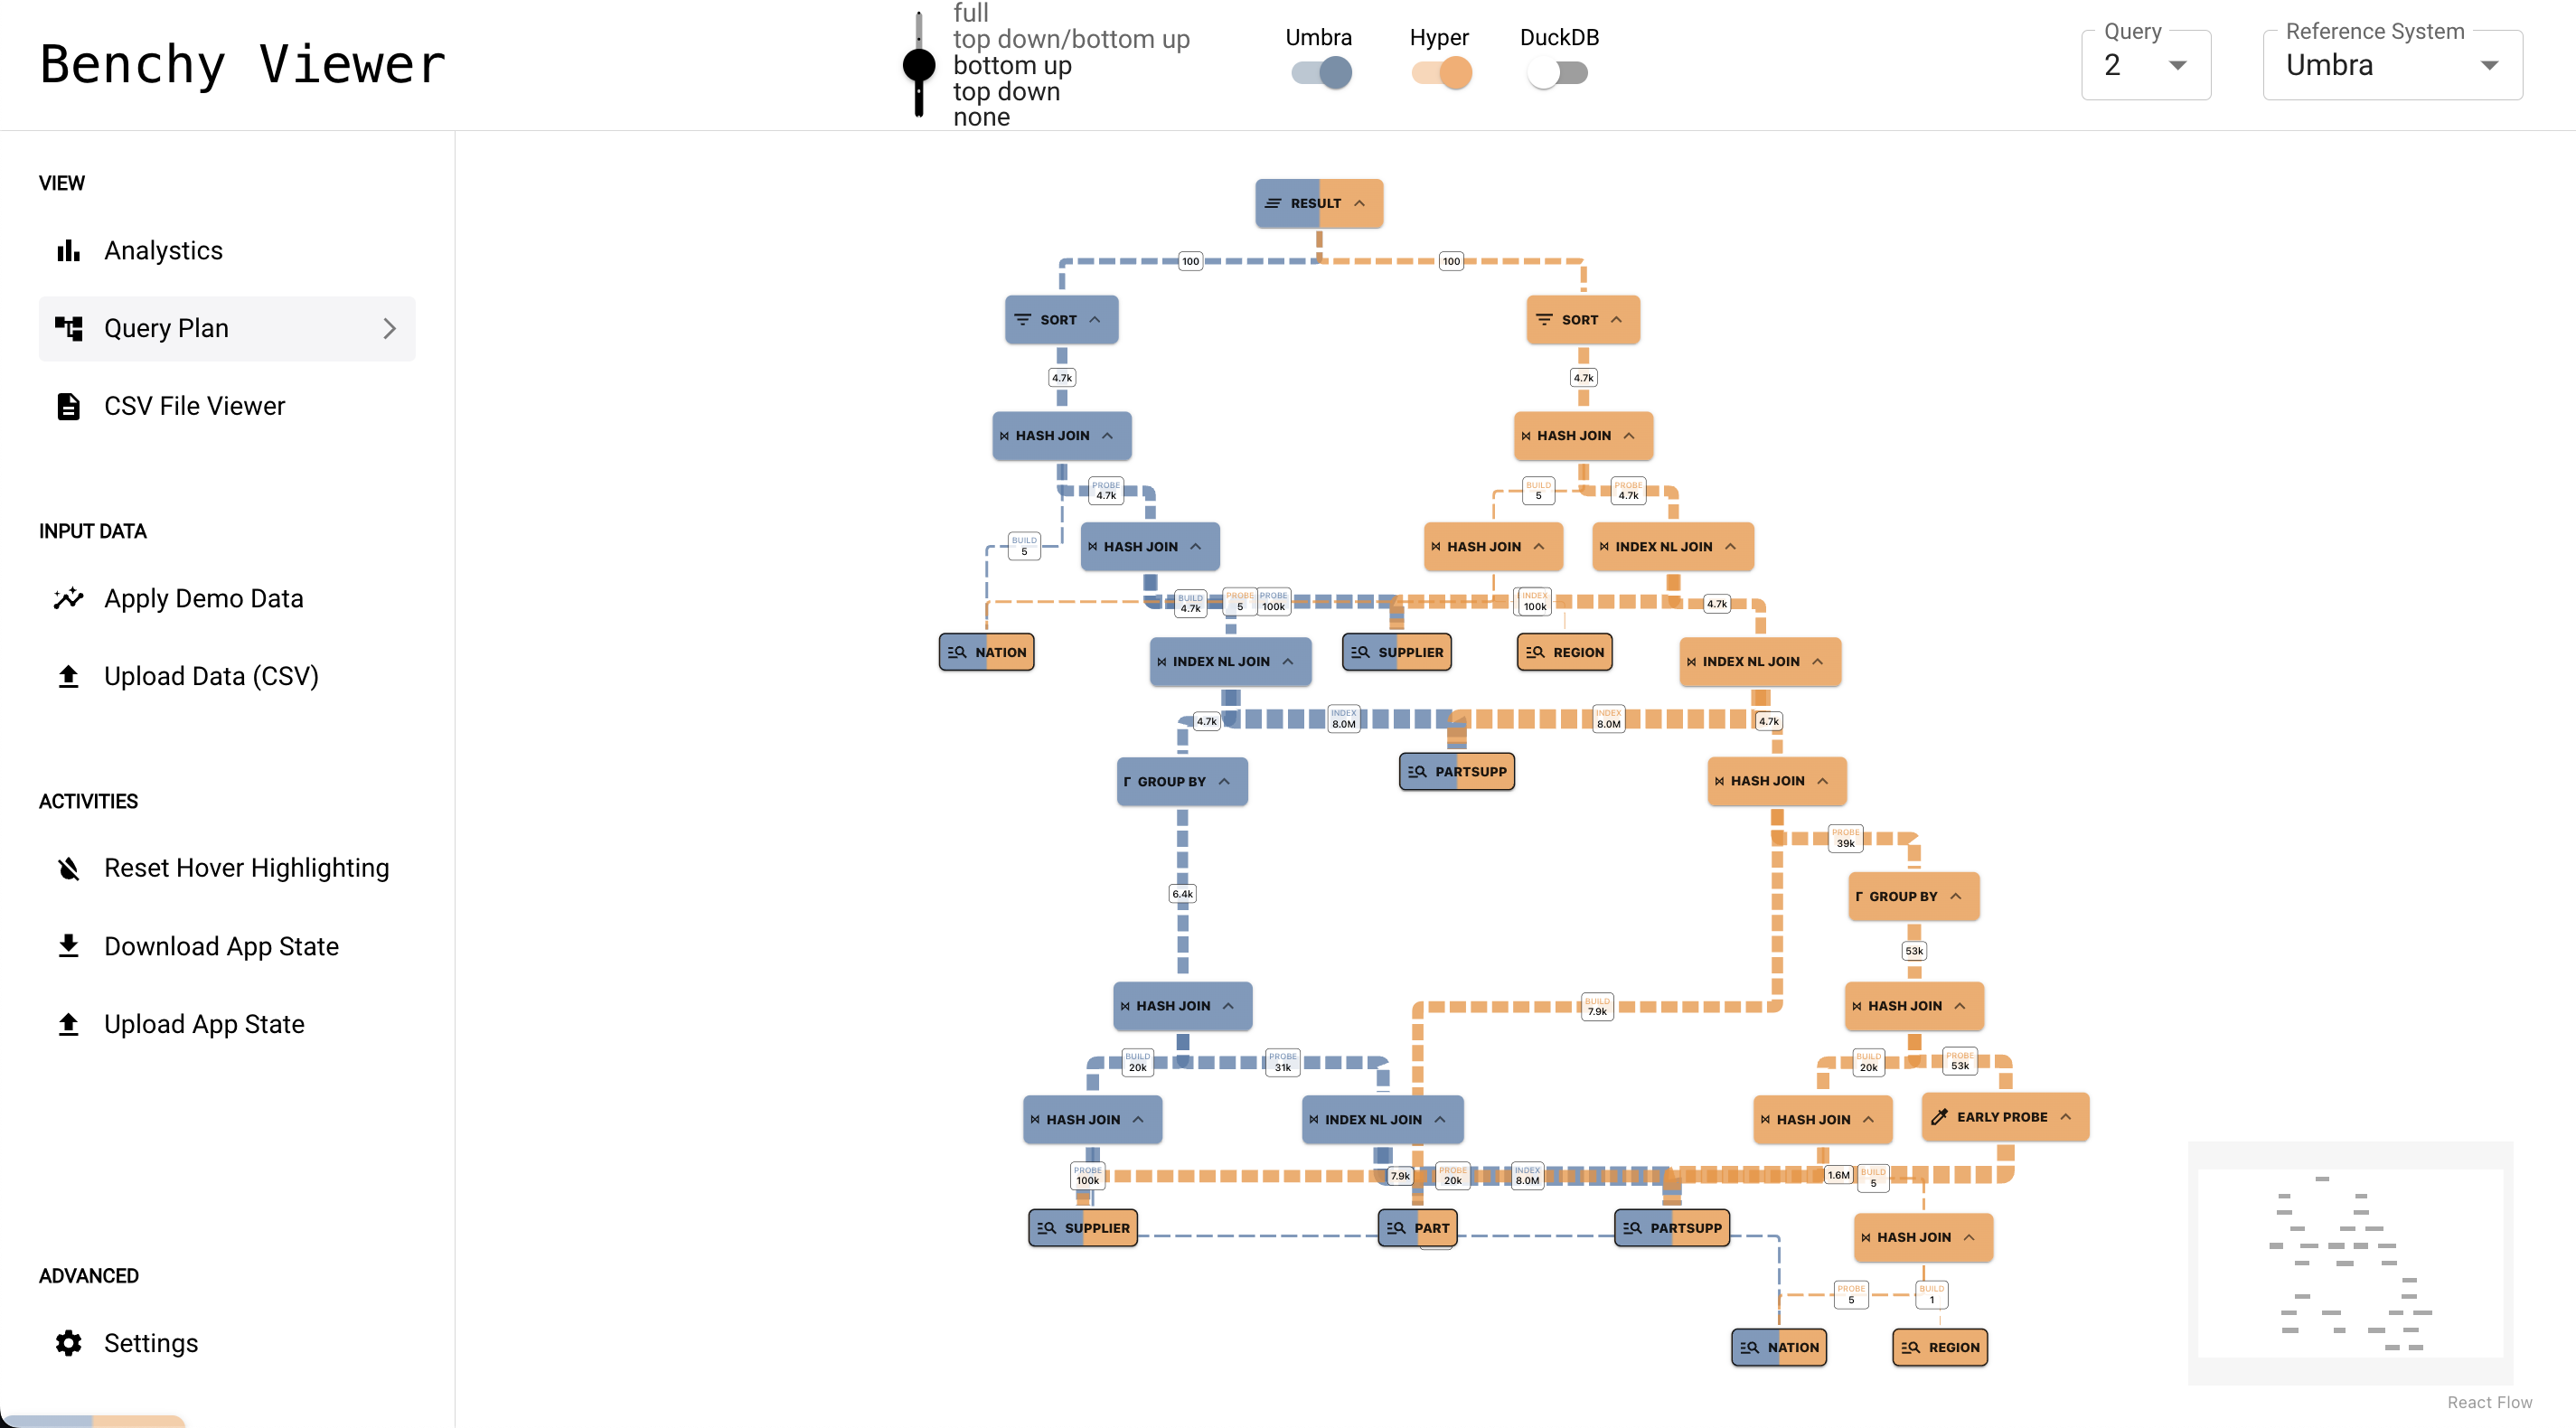
\includegraphics[width=\linewidth]{figures/app-query-plan.png}
      \caption{Query Plan View.}
        \label{fig:abstract-query-plan}
    \end{subfigure}
    \hspace{0.5cm} % Adjust the horizontal space between the figures
    \begin{subfigure}[b]{0.3\linewidth}
      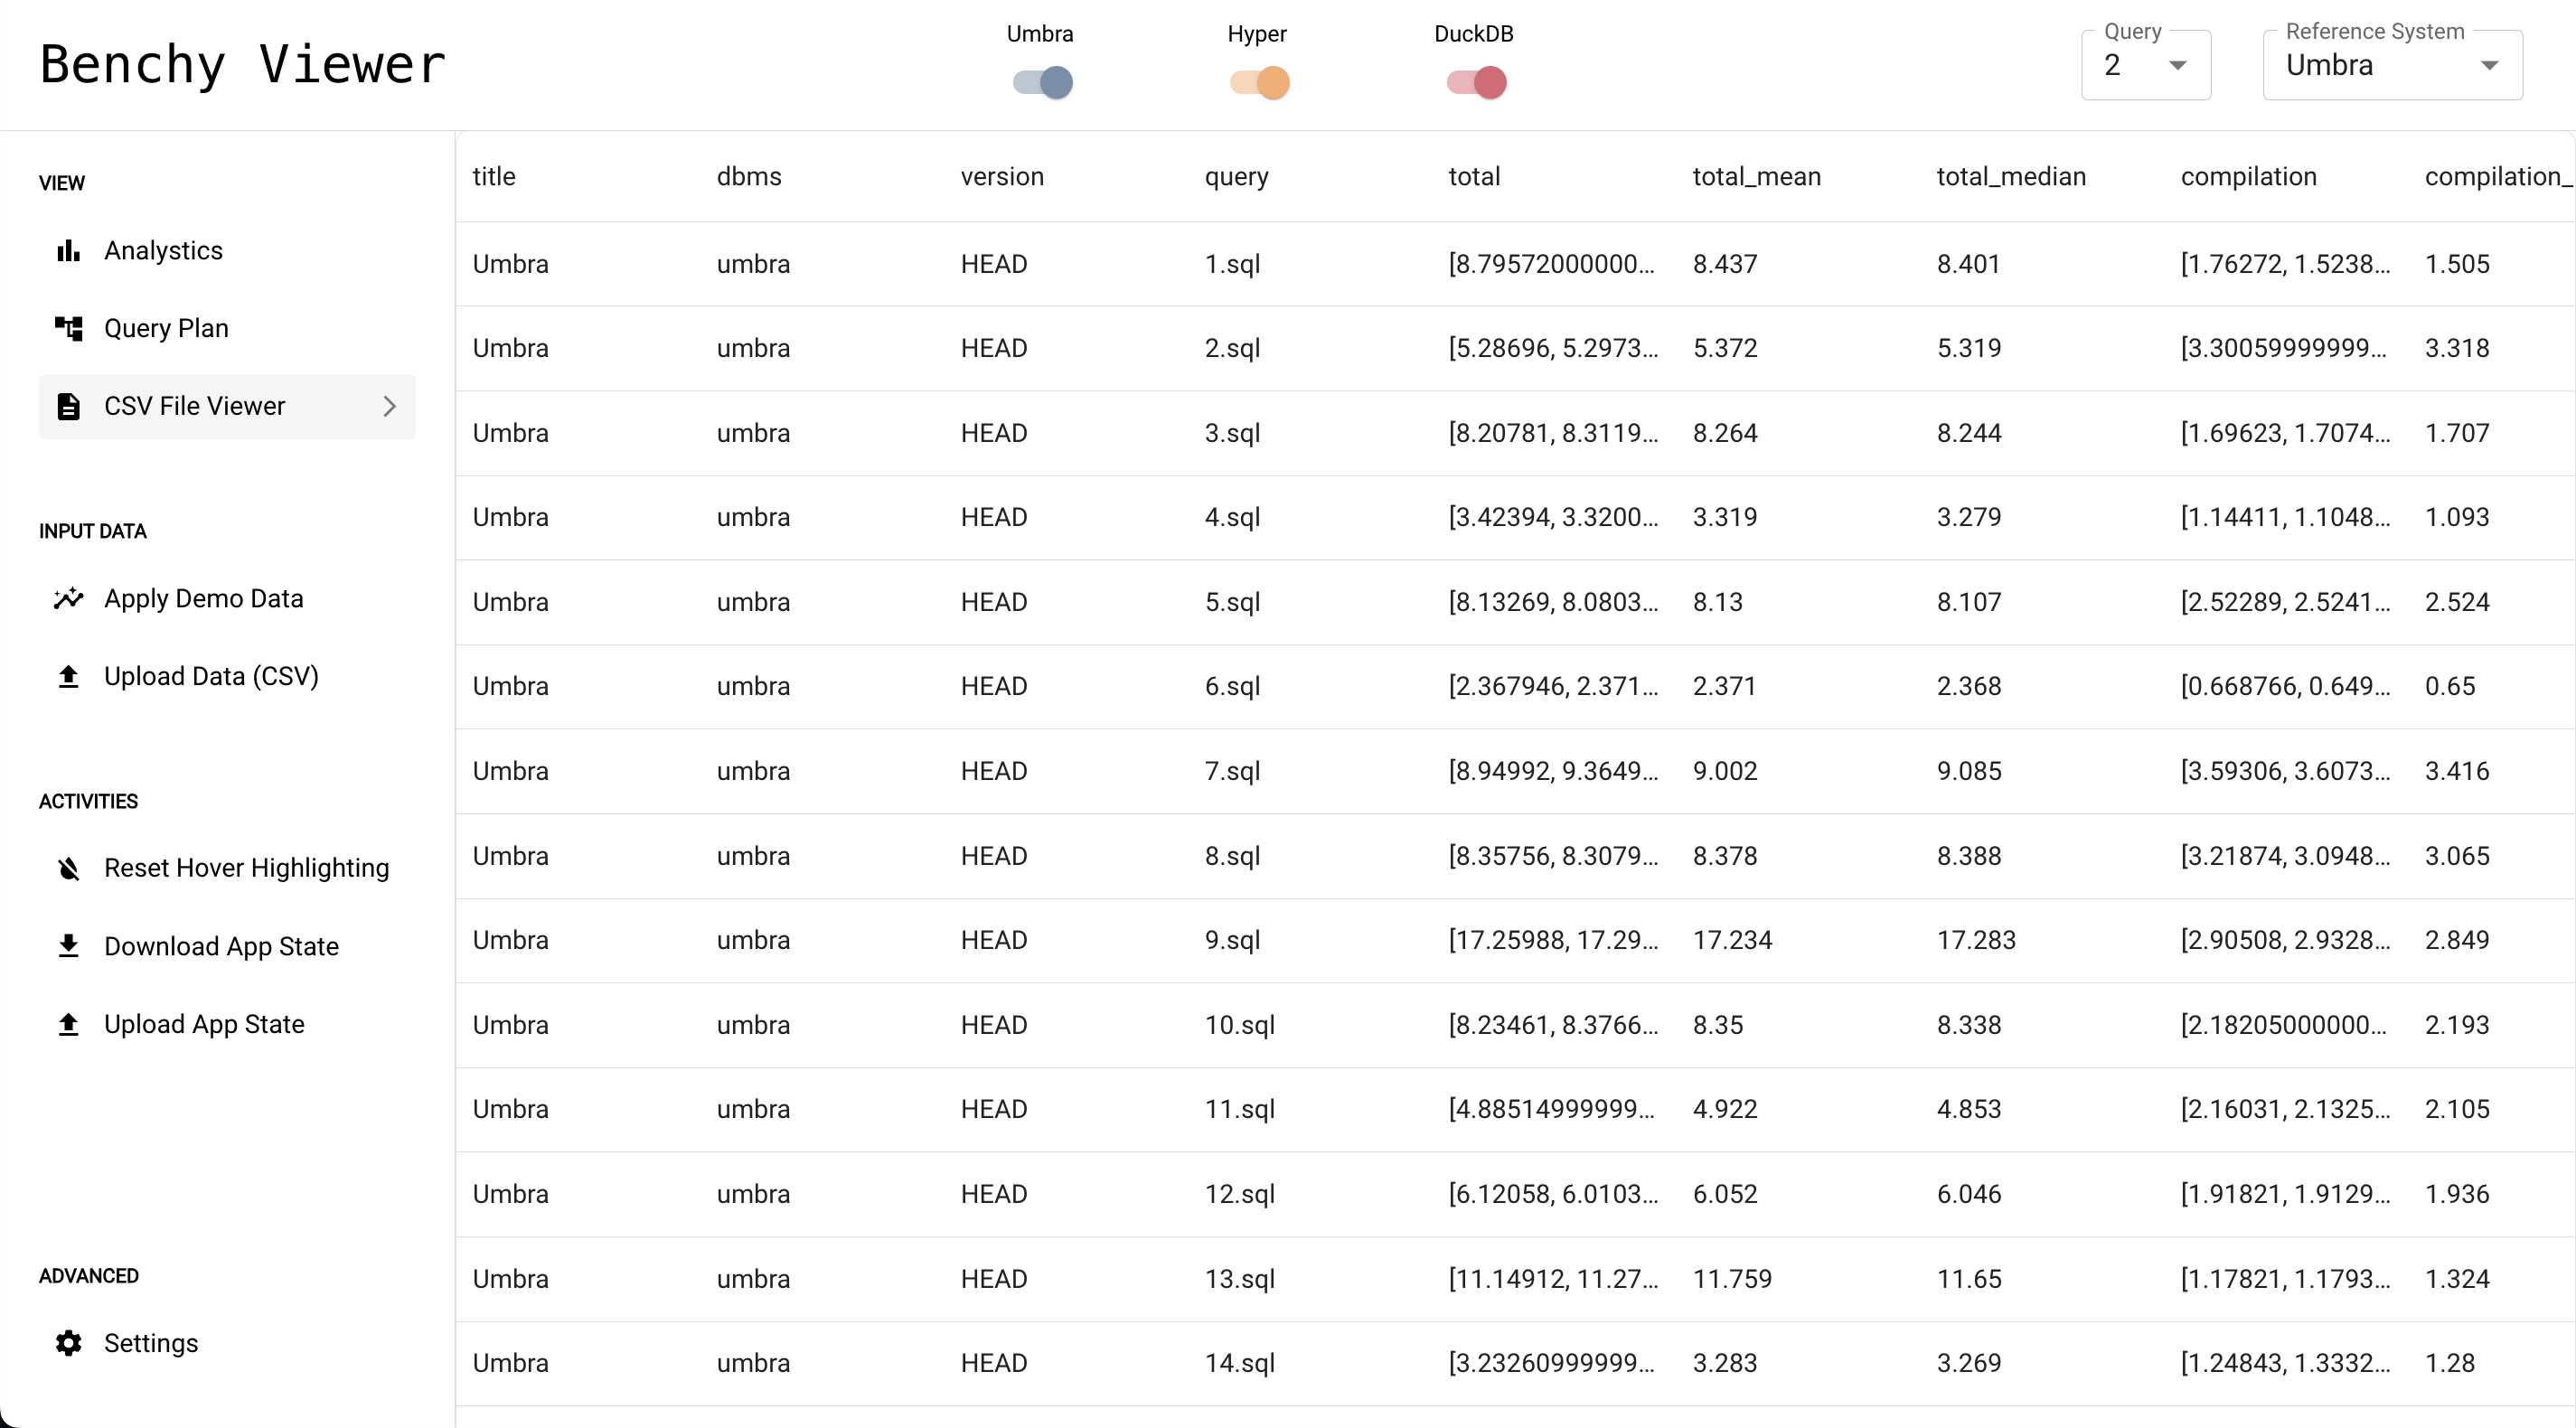
\includegraphics[width=\linewidth]{figures/app-data-viewer.png}
      \caption{Input File Viewer.}
        \label{fig:abstract-data-viewer}
    \end{subfigure}
    \caption{Benchy Viewer: Tool for analyzing performance measurements of database systems through interactive visualizations.}
    \label{fig:abstract}
  \end{figure}

%   In the ever-evolving landscape of database systems,

% This master thesis introduces the Benchy Viewer, a web-based serverless application designed for interactive exploration and analysis of performance data from various database systems. The primary objective is to empower database engineers by providing an intuitive platform for in-depth query execution analysis.\\
% We focus on consolidating a variety of interactive diagrams that portray diverse information content, aiming to elevate the interpretation of profiling data in database systems. The scope delineates the primary questions guiding the investigation, with a focus on the design and development of the Benchy Viewer application, as well as the exploration of statistical methods for analyzing performance data in database systems.


% The thesis structure navigates through related work, theoretical foundations, and the implementation of the Benchy Viewer. It scrutinizes the theoretical underpinnings of database systems, delves into datasets and data structures, and unveils the intricacies of implementation, emphasizing features, interaction capabilities, and design guidelines.

Embarking on the intricate journey of database performance optimization, this thesis underscores the pivotal role of performance analysis in benchmark data. A foundational understanding of system intricacies is paramount for overall performance enhancement. Recognizing the indispensability of visualizations in this analytical process, our work introduces the Benchy Viewer, a web-based serverless application meticulously designed to elevate the analysis of performance benchmark data.

Our main focus is on delivering interactive visualizations through an intuitive user interface, creating an environment where database developers can seamlessly navigate and interpret benchmark data. Developed using React, the Benchy Viewer stands out for its flexibility and the degree of interaction embedded in its intuitive user interface, empowering developers to dynamically explore benchmark data. It offers diverse perspectives, allowing users to view performance metrics from various angles, including a comparison perspective of query plans across different system instances, adding a layer of depth to performance analysis.

Built on an extensible architecture, the Benchy Viewer paves the way for future improvements. Its adaptability enables the incorporation of additional visualizations and analytical perspectives. 
In essence, the Benchy Viewer emerges as a transformative tool, achieving varied perspectives through interactive visualizations and an intuitive user interface, while its extensible architecture opens avenues for continuous enhancement.






